\documentclass[]{article}
\usepackage[a4paper, total={15cm,23cm}]{geometry}
\usepackage{fancyhdr}
\usepackage{graphicx}
\usepackage{amsmath}
\usepackage{amssymb}
\usepackage{xcolor}
%opening
\title{PH 223 Week 2}
\author{Benjamin Bauml}
\date{Winter 2024}
\pagestyle{fancy}
\rhead{PH 223}
\chead{Winter 2024}
\lhead{Week 2}

%Custom Quotation Command
\newcommand{\excerpt}[1]{\colorbox{lightgray}{\parbox{14.8cm}{#1}} \\}

\begin{document}

\maketitle

\begin{center}
	Activities 2 and 3 are borrowed/adapted from Chapter 23 of \textit{Physics for Scientists and Engineers}, as well as its associated \textit{Student Workbook}.

\end{center}
\section*{Activity 1}%6

(a) To derive Kepler's 3rd law, one can start by equating the gravitational force and the centripetal force necessary for uniform circular motion:
\[
F_{g} = \frac{GMm}{r^{2}} = \frac{4\pi^{2}mr}{T^{2}} = F_{c},
\]
where we have made use of the substitution $ \omega = 2\pi f = \frac{2\pi}{T} $. Let us model protons and electrons as classical point particles, with the electron in uniform circular motion around the proton. How would we change the above condition to account for the effects of charge?

% To reveal the solution, delete "\phantom{\parbox{\textwidth}{" from the beginning, and "}}" from the end.
\iffalse
\phantom{\parbox{\textwidth}{
To account for the Coulomb interaction, we need to insert a term of the form
\[
\frac{Kq_{1}q_{2}}{r^{2}}.
\]
The charge on an electron is $ -e $, and the charge on a proton is $ +e $, which would make the force between the two particles attractive. As such, the magnitude of the Coulomb force between a proton and an electron (which is $ \frac{Ke^{2}}{r^{2}} $) adds to the attractive gravitational force to create the net centripetal force. Our equation should be
\[
\frac{GMm}{r^{2}} + \frac{Ke^{2}}{r^{2}} = \frac{4\pi^{2}mr}{T^{2}}.
\]
}}
\fi


(b) Let $ e = 1.60\times10^{-19} $ C be the magnitude of charge on a proton or electron, $ M = 1.67\times10^{-27} $ kg be the mass of the proton, and $ m = 9.11\times10^{-31} $ kg be the mass of an electron. Compare $ GMm $ and $ Ke^{2} $ in terms of order of magnitude (the powers of 10 in scientific notation). Are they similar, or is one much larger than the other?

% To reveal the solution, delete "\phantom{\parbox{\textwidth}{" from the beginning, and "}}" from the end.
\iffalse
\phantom{\parbox{\textwidth}{
Considering only orders of magnitude, $ G \sim 10^{-11} $ Nm$ ^{2}/ $kg$ ^{2} $, $ M \sim 10^{-27} $ kg, and $ m \sim 10^{-30} $ kg (because the leading 9 in $ 9.11\times10^{-31} $ is close to another order of magnitude). As such, $ GMm \sim 10^{-68} $ Nm$ ^{2} $. For the electric terms, $ K \sim 10^{10} $ Nm$ ^{2}/ $C$ ^{2} $ (because the leading 9 in $ 9\times10^{9} $ is close to another order of magnitude) and $ e \sim 10^{-19} $ C. Thus, $ Ke^{2} \sim 10^{-28} $ Nm$ ^{2} $. Clearly, $ GMm \ll Ke^{2} $ (by about 40 orders of magnitude). For those who want an exact calculation:
\[
\begin{split}
	GMm & = (6.67\times10^{-11}\text{ Nm}^{2}/\text{kg}^{2})(1.67\times10^{-27}\text{ kg})(9.11\times10^{-31}\text{ kg}) = 1.01\times10^{-67} \text{ Nm}^{2}; \\
	Ke^{2} & = (9\times10^{9}\text{ Nm}^{2}/\text{C}^{2})(1.60\times10^{-19}\text{ C})^{2} = 2.30\times10^{-28}\text{ Nm}^{2}.
\end{split}
\]
We were off by an order of magnitude in the first expression, because $ 6.67\times1.67 = 11.1389 \sim 10 $. Still, $ GMn \ll Ke^{2} $ (by 39 orders of magnitude). We can safely ignore the contribution of the gravitational force to this situation.
}}
\fi


(c) Take your modified expression from part (a) and remove the gravitational term. If we take the distance between the proton and the electron to be $ r = 5.29\times10^{-11} $ m (the Bohr radius), then what order of magnitude is the rotational frequency of the electron? What SI prefix should I be appending to hertz when I express this frequency?

% To reveal the solution, delete "\phantom{\parbox{\textwidth}{" from the beginning, and "}}" from the end.
\iffalse
\phantom{\parbox{\textwidth}{
Without the gravitational term, our expression becomes
\[
\frac{Ke^{2}}{r^{2}} = \frac{4\pi^{2}mr}{T^{2}} = 4\pi^{2}mrf^{2}.
\]
Solving for frequency, we find
\[
f = \sqrt{\frac{Ke^{2}}{4\pi^{2}mr^{3}}}.
\]
We already know that $ Ke^{2} \sim 10^{-28} $ Nm$ ^{2} $ and $ m \sim 10^{-30} $ kg. Furthermore, $ \pi^{2} \sim 10 $, and because $ 5^{3} = 125 $, we should be choose $ r^{3} \sim 10^{-31} $ instead of $ 10^{-33} $. Finally, let us consider 4 to be on the order of 1. All together, this means
\[
\frac{Ke^{2}}{4\pi^{2}mr^{3}} \sim \frac{10^{-28}\text{ Nm}^{2}}{10\times10^{-30}\times10^{-31}\text{ kg m}^{3}} = 10^{32}\text{ s}^{-2}.
\]
Thus $ f \sim 10^{16} $ Hz, which would be on the order of ten petahertz. An exact calculation shows
\[
f = \sqrt{\frac{2.30\times10^{-28}\text{ Nm}^{2}}{4\pi^{2}(9.11\times10^{-31}\text{ kg})(5.29\times10^{-11}\text{ m})^{3}}} \approx \sqrt{4.32\times10^{31}\text{ s}^{-2}} \approx 6.57\times10^{15}\text{ Hz}
\]
We were off by one order of magnitude for discounting the full effect of certain minute details. The frequency is on the order of one petahertz.
}}
\fi
%  s\fi

\section*{Activity 2}%6
At each of the dots, use a \textbf{black} pen or pencil to draw and label the electric fields $ \vec{E}_{1} $ and $ \vec{E}_{2} $ due to the two point charges. Make sure that the \textit{relative} lengths of your vectors indicate the strength of each electric field. Then use a \textbf{red} pen or pencil to draw and label the net electric field $ \vec{E}_{net} $ at each dot.

\begin{center}
	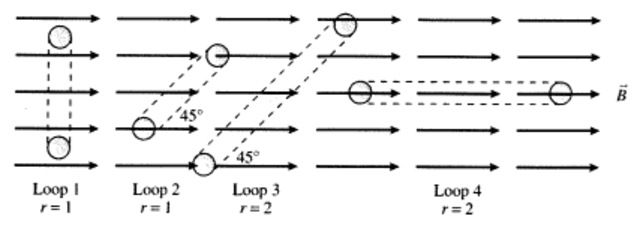
\includegraphics[scale=0.5]{A1}
	%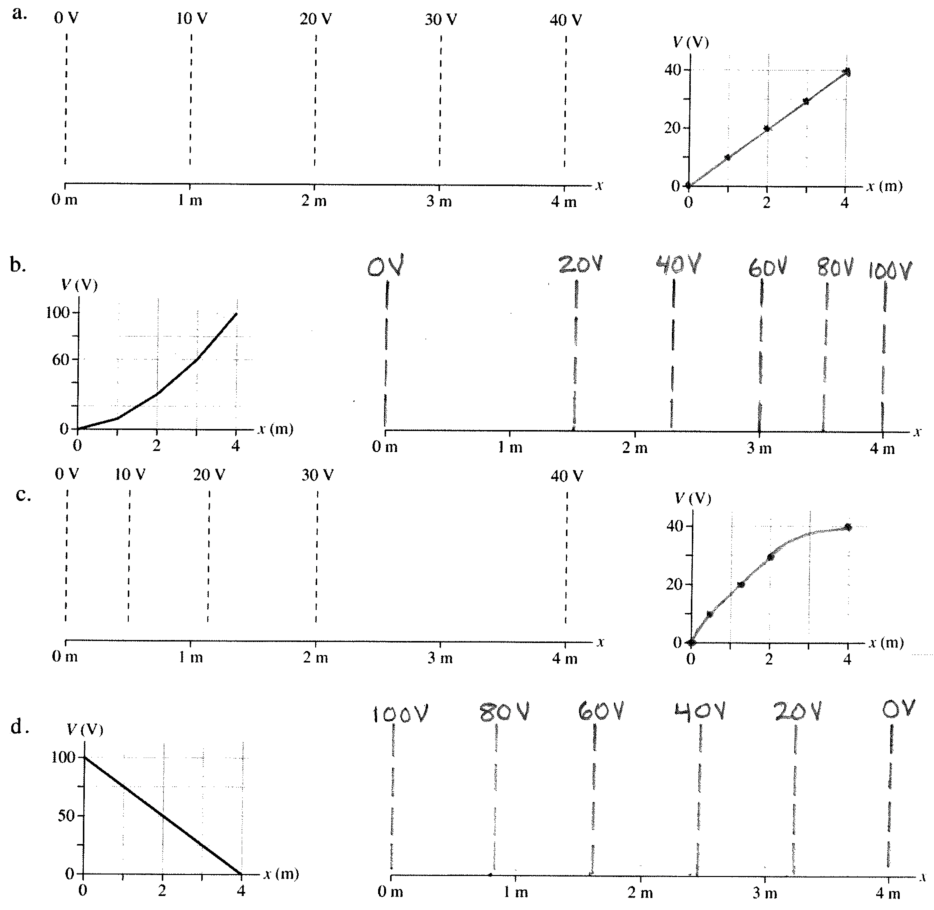
\includegraphics[scale=0.5]{A1Sol}%Solution
\end{center}
% To reveal the solution, delete "\phantom{\parbox{\textwidth}{" from the beginning, and "}}" from the end.
\iffalse
\phantom{\parbox{\textwidth}{
In (b), the $ \vec{E}_{1} $ vectors now point toward $ q_{1} $, as it is negative.
}}
\fi

\section*{Activity 3}%6
For each of the figures, use dots to mark any point or points (other than infinity) where $ \vec{E} = \vec{0} $.

\begin{center}
	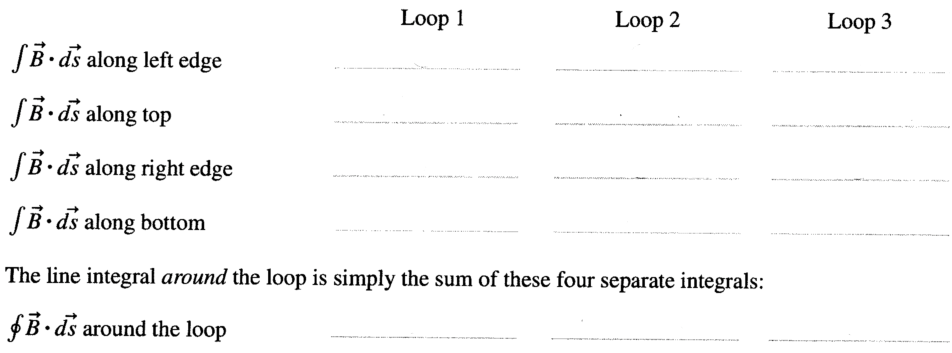
\includegraphics[scale=0.5]{A2a}
	%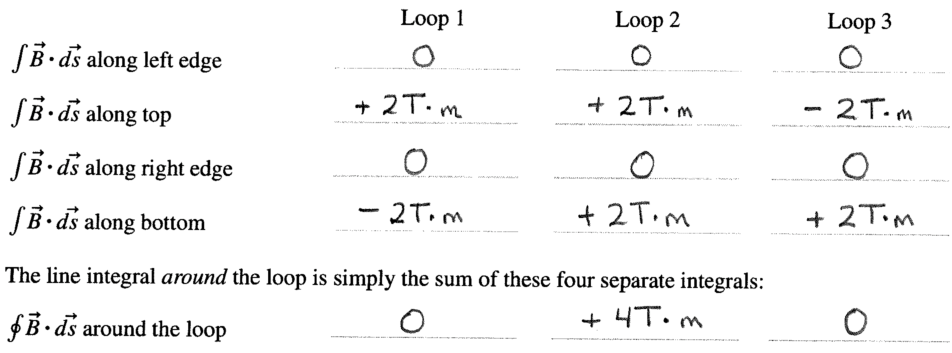
\includegraphics[scale=0.5]{A2aSol}%Solution
\end{center}
% To reveal the solution, delete "\phantom{\parbox{\textwidth}{" from the beginning, and "}}" from the end.
\iffalse
\phantom{\parbox{\textwidth}{
Let the charge on the right be $ q $. The charge on the left is $ 4q $, so its electric field is four times as strong at the same distance. The net electric field can only be zero where both constituent fields work against each other, so there cannot be a zero to the right of $ q $ or to the left of $ 4q $, where their fields combine to be stronger. Somewhere in between the two, we want the field to satisfy
\[
\frac{4Kq}{r_{4q}^{2}} = \frac{Kq}{r_{q}^{2}} \implies 4 = \frac{r_{4q}^{2}}{r_{q}^{2}} \implies 2 = \frac{r_{4q}}{r_{q}}.
\]
The point of zero electric field occurs at a position twice as far away from $ 4q $ as from $ q $, which occurs at the indicated tick mark.
}}
\fi
\begin{center}
	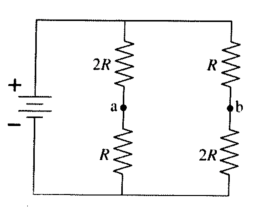
\includegraphics[scale=0.5]{A2b}
	%\includegraphics[scale=0.5]{A2bSol}%Solution
\end{center}
% To reveal the solution, delete "\phantom{\parbox{\textwidth}{" from the beginning, and "}}" from the end.
\iffalse
\phantom{\parbox{\textwidth}{
By changing $ q $ to $ -q $, we have switched the direction of its electric field. Now, the two fields are parallel in the space between the charges, so there cannot be a zero there. To the left of $ 4q $, the field point is closer to the larger charge, so the electric field from $ -q $ has no hope of counteracting the larger charge's field. We look to the region to the right of $ -q $, where we must again satisfy
\[
\frac{4Kq}{r_{4q}^{2}} = \frac{Kq}{r_{q}^{2}} \implies 4 = \frac{r_{4q}^{2}}{r_{q}^{2}} \implies 2 = \frac{r_{4q}}{r_{q}}.
\]
We still find the point of zero electric field to be at a location twice as far from $ 4q $ as from $ -q $, but now that occurs at the indicated tick mark instead of between the two charges.
}}
\fi



\end{document}
